\documentclass[a4paper]{article}

\usepackage{alltt}
\usepackage{graphicx}
\usepackage{fancyvrb,relsize}


\setlength\textwidth{5.0in}
\setlength\oddsidemargin{0.5in}
\setlength\evensidemargin{0.5in}
%\setlength\parindent{0.25in}
%\setlength\parskip{0.25in} 

\newcommand{\urlb}{\footnotesize\begin{alltt}} 
\newcommand{\urle}{\end{alltt}\normalsize} 
\newcommand{\exampleb}{\small\begin{alltt}} 
\newcommand{\examplee}{\end{alltt}\normalsize} 
\renewcommand{\familydefault}{\sfdefault}
\newcommand{\xmlv}[1]{\textbf{\textless#1\textgreater}} 
\newcommand{\xml}[1]{\textless#1\textgreater} 
\newcommand{\dnsdb}{DNS\textsuperscript{2db}\hspace{3pt}} 
\newcommand{\HRule}{\rule{\linewidth}{0.5mm}}


\begin{document}
\begin{titlepage}
 
\begin{center}
 

 

 
\textsf{\large  .SE (The Internet Infrastructure Foundation)}\\[0.5cm]
 
 
% Title
\vspace{3.5cm}

{ \huge \bfseries \dnsdb User's manual }\\[0.4cm]
 v2.2.1 
 


 

 
\vfill
 
% Bottom of the page
{\large January 2010}
 
\end{center}
 
\end{titlepage}

\newpage
\setcounter{page}{2}
\section{Preface}
This user's manual has been written to help those who decide to run the \dnsdb system. 
More information about building or installing \dnsdb and developer information such as an xml-format specification and an interface specification of the php files can be found at:

\verb|http://opensource.iis.se/trac/dns2db/|    

 

The man pages for tracedns and dns2sqlite may be useful for those who would like to customize the perl job control daemon or roll their own.
Information about third party software used in \dnsdb can be found at the following locations.
\begin{center}
    \begin{tabular}{ | l | p{9cm} |}
    \hline
libtrace		&	http://research.wand.net.nz/software/libtrace.php\\ \hline

ldns			&	http://www.nlnetlabs.nl/ldns/\\ \hline

SQLite3			&    http://www.sqlite.org/\\ \hline

Adobe Flex3		&	http://www.adobe.com/products/flex/\\ \hline

    \end{tabular}
\end{center}


\newpage
\tableofcontents
\newpage



\section{Introduction}
\dnsdb is a DNS query statistics and analysis application.

It is used to monitor and analyze traffic on DNS servers, especially during traffic peaks where it is
helpful to know the cause of the peak. It may also be used to identify serious errors in DNS
configuration which causes unnatural DNS traffic. 

The design of \dnsdb makes it possible to get this information within a few 
minutes and could be extended to report near realtime information on
for example load and various predefined patterns. It may also be used to 
do statistical analysis on DNS traffic over time.
    

\section{Overview}
\dnsdb consists of two main parts, a collector backend and a GUI.
The backend collects and converts raw pcap data from a network into sqlite3 databases. Collecting
and converting is done in two separate processes, tracedns for capturing and dns2sqlite for parsing
and storing to database. If there is a need to store pcap data for later reference this can best be done
by capturing pcap to disk before conversion. The data collecting is done in close proximity to the
dns server and the collected information is made accessible to the user through a web based GUI
using the XML API.

The GUI is written as an Adobe Flex application that runs in any flash enabled web browser. The
Flex GUI can get information from the databases through a php script that specifies and limits the
information available to the GUI. The GUI application is served completely from the server and no
additional software is needed on the client.
Figure 1 is a description of a complete \dnsdb implementation on a separate packet capturing
server that listens on incoming and outgoing traffic to a DNS server. The setup for sniffing traffic
can be done with port forwarding in a connected switch, with a transparent ethernet splitter or by
other means. It can also be done on the DNS server itself but this is not recommended. The \dnsdb
system is started and stopped by a wrapper script named dns2db.

\newpage
\section{The Collector nodes}
\subsection{Overview}

The following files are part of a \dnsdb collector node:


\begin{center}
    \begin{tabular}{ | l | p{7cm} |}
    \hline
    \textbf{File} & \textbf{Description}  \\ \hline
    \verb|tracedns|&                    The input module of \dnsdb\\ \hline

    \verb|dns2sqlite|&                  The output module of \dnsdb\\ \hline

    \verb|/etc/dns2db.conf| &           Configuration file\\ \hline

    \verb|/etc/init.d/dns2db| &      Init script\\ \hline

    \verb|/usr/bin/dns2db.pl|     &     Process control script
    
     (used by /etc/init.d/dns2db)\\ \hline

    \verb|dns2dbnode.php|        &      php backend on each collector node\\ \hline

    \verb|dns2dbnode_conf.php|      &   php config file for the collector node\\ \hline

    \end{tabular}
\end{center}

The dns2db init script reads configuration parameters in /etc/dns2db.conf and calls
/usr/bin/dns2db.pl to start the tracedns and the dns2sqlite binary with command line arguments from
the dns2db.conf file. Arguments to the wrapper script are start\verb%|%stop. Configuration parameters for
the processes are set by the wrapper during startup and cannot be changed during run time.
Optionally the start script starts a separate capturing process to store pcap data and runs the
\dnsdb processes after every new pcap file.
The tracedns process reads from the configured input and writes to stdout. Input can be any file or
interface that libtrace can handle. Eg ``pcapint:eth0'' for the first network interface on a Linux
system or ``pcapfile:/a-file.pcap'' for a pcap file on a local drive.
The dns2sqlite process listens to stdin and creates the databases in the path set in dns2db.conf.

\subsection{The dns2db.pl job control daemon}
The dns2db.pl job control daemon is usually started by the initscript dns2db and is the 
process that starts tracesplit to generate pcap files and then tracedns and dns2sqlite to 
generate sqlite databases for each interval. It also indexes the databases.
The dns2db.pl script is configure by /etc/dns2db.conf. Configuration parameters for
the processes are set up during startup and cannot currently be changed during run time.

\subsection{Initscript}
The dns2db init script reads configuration parameters in /etc/dns2db.conf and calls
/usr/bin/dns2db.pl which starts the tracedns and the dns2sqlite binary with command line arguments from
the dns2db.conf file. Arguments to the wrapper script are start\verb%|%stop. 
This script may need to be customized to your particular operating system.

\subsection{The tracedns command}
The tracedns process reads from the configured input and writes to stdout. Input can be any file or
interface that libtrace can handle. Eg ”pcapint:eth0” for the first network interface on a Linux
system or ”pcapfile:/a-file.pcap” for a pcap file on a local drive.

\subsection{The dns2sqlite command}
The dns2sqlite process listens to stdin and creates the databases in the path set in dns2db.conf.

\subsection{The configuration file}

Heres an example configuration file (/etc/dns2db.conf).

\begin{Verbatim}[fontsize=\relsize{-1},numbers=left]
## dns2db pid file
pidfile=/var/run/dns2db.pid

## Name of the DNS server. Parameter is used first in filename 
## when creating tcpdump files and sql files.
server="servername"

## Ramdisk where database is created and indexed
workdir=/tmp/workdir

## Final directory where databases and pcap files are stored
# make sure path ends with trailing "/"
destdir=/tmp/outputdir/

## chmod finished files to serve from apache
user=www-apache-httpd

## Name of the network interface to monitor
interface=eth0

## How often to rotate dump file, in seconds
interval=300

## Keep pcap data
keeppcap=YES

## Compress pcap data
compresspcap=YES

## BSD libtrace promiscous interface hack 
# uses a tcpdump session on port 100 to keep the interface 
# in promisc mode because tracesplit seems to be unable 
# to do so on bsd
bsdpromischack=NO

## path to the tcpdump binary
tcpdump=tcpdump

## path to the tracesplit binary
# tracesplit is distributed in the tools folder of the libtrace 
# library make sure it's built and installed.
tracesplit=/usr/local/bin/tracesplit

### choose a packet filter:
## collect TCP and UDP, requests and responses:
filter="port 53"

## create sqlite index
index="create index ix_src_addr on q (src_addr);create index 
domain on q (rr_lvl2dom,rr_lvl1dom);create index ix_rr_type 
on q (rr_type); create index if not exists resanddom on q 
(rr_cname,src_addr,rr_type);"
\end{Verbatim}

The fields that must be changed to have a working collector 
are workdir, destdir, user and interface.

\begin{itemize}
\item The parameter \textbf{workdir} specifies a working directory for optimal performance this 
should be placed on a ramdisk with enough space for pcap files and database 
files for three peek intervals.

\item The  \textbf{destdir} path points to the path where the database files are to be stored.
\item The  \textbf{user} parameter specifies the user that will own the resulting files. 
This should normally be the web server user to allow the databases to be 
accessed by the php scripts.
\item The  \textbf{interface} parameter specifies which network interface to listen on i.e. eth0.
\item The \textbf{filter} parameter can be used to specify a berkely packet filter 
string to trancedns that can be used to filter the output to specific ports 
and/or hosts. This is usually "port 53" to only see dns traffic but could also 
include filters to i.e. filter out dns queries from the dns server itself ("port 53 and not host 192.168.0.1").
\end{itemize}

\subsection{The PHP scripts}
The file dns2db\_node.php serves results through a web server to dns2db.php 
on the gui server which may or may not be the same machine. 

Normally the dns2db\_node.php script uses the database path 
from /etc/dns2db.conf but in cases where the web server is running chrooted 
it's recommended to rename the file dns2dbnode\_conf.php.example into 
dns2dbnode\_conf.php and to change the path within to correspond to 
the destdir of /etc/dns2db.conf.


\newpage
\section{The gui server}
The following files are part of the GUI server:

\begin{center}
    \begin{tabular}{ | l | p{7cm} |}
    \hline
    \textbf{File} & \textbf{Description}  \\ \hline
    \verb|index.php|&                    html part of the Adobe Flex application\\ \hline

    \verb|dns2db.swf|&                  the Adobe Flex application\\ \hline

    \verb|dns2db.php| &           php backend for the Flex application\\ \hline

    \verb|dns2db_conf.php| &      config file for the GUI\\ \hline

    \verb|reversedb.db3|     &     reverse lookup cache for the GUI\\ \hline

  

    \end{tabular}
\end{center}
	


The GUI consists of a flash application, a set of php scripts and a reverse DNS 
lookup cache database. When the flash application is loaded in the users webbrowser 
it will default to presenting toplists for current time in UTC minus 5 minutes.

Note: reversedb.db3 must be writable by the web server user, also applies to 
the catalogue containing the reversedb.db3.

\subsection{The PHP configuration file}
The file dns2db\_conf.php is the only file that needs to be changed on the GUI server.
The default file looks like this:

\begin{Verbatim}[fontsize=\relsize{-1},numbers=left]
<?php
########## urls for the swf and dns2db.php files
#
#  the default relative paths below should be fine for most users
$swf = "dns2db.swf";
$url = "dns2db.php";


########## reverse lookup cache 
# this specifies the location of the name lookup cache database
# make sure both this file and the directory it's in is 
# writable by the web server user
$database = "reversedb.db3";

$nodes = array (  # start nodelist

##########  nodelist   #########################################################
# add each collector node to the $nodes array here using a 
# line like the example below
# make sure the 'url' is reachable by the dns2db script and that 
# the 'name' is free of any whitespace characters
#
    array(  'name' => 'x' , 
            'dnsname' => 'x.example.comm', 
            'url' => 'http://x.example.comm/dns2db/test/dns2dbnode.php', 
            'displayname'=>'X', 
            'description'=>'the server X'),
            
#   array(  'name' => 'y' , 
            'dnsname' => 'y.example.comm', 
            'url' => 'http://y.example.comm/dns2db/dns2dbnode.php', 
            'displayname'=>'Y', 
            'description'=>'the server Y'),

); 	# end nodelist


$rrstats = array (  # start rrstats
##########  rrstats   #########################################################
#
#  this array provides data for coloring the rrtypes display in the gui
#  deviation controls the deviation where coloring occurs

   array( 'name' => 'A' , 'percent' => '49', 'deviation' => '4'),
   array( 'name' => 'MX' , 'percent' => '23', 'deviation' => '3'),
   array( 'name' => 'AAAA' , 'percent' => '13', 'deviation' => '2'),
   array( 'name' => 'NS' , 'percent' => '10', 'deviation' => '2'),
   array( 'name' => 'TXT' , 'percent' => '1', 'deviation' => '0.5'),
   array( 'name' => 'DS' , 'percent' => '0.9', 'deviation' => '0.5'),
   array( 'name' => 'A6' , 'percent' => '0.8', 'deviation' => '0.5'),
   array( 'name' => '*' , 'percent' => '0.4', 'deviation' => '.3'),
   array( 'name' => 'SOA' , 'percent' => '0.2', 'deviation' => '.2'),
   array( 'name' => 'SRV' , 'percent' => '0.1', 'deviation' => '0.1'),
   array( 'name' => 'SPF' , 'percent' => '0.1', 'deviation' => '0.1'),
   array( 'name' => 'PTR' , 'percent' => '0.1', 'deviation' => '0.1'),
   array( 'name' => 'CNAME' , 'percent' => '0.1', 'deviation' => '0.1'),
   array( 'name' => 'DNSKEY' , 'percent' => '0.1', 'deviation' => '0.1'),
   array( 'name' => 'RRSIG' , 'percent' => '0.1', 'deviation' => '0.1'),
   array( 'name' => 'NSEC' , 'percent' => '0.1', 'deviation' => '0.1'),
                                                
);      # end rrstats
?>
\end{Verbatim}

The most important part of this configuration file is the nodelist where you configure you nodes.
Each node needs to have a name,dnsname,url,displayname and description.
\begin{itemize}
\item \textbf{name} specifies a short unique name for the node used in communication between the flex gui client and the gui server.
\item \textbf{dnsname} specifies the dnsname of the node this is not currently used in the gui.
\item \textbf{url} specifies the http url where the nodes dns2dbnode.php script can be accessed by the gui server.
\item \textbf{displayname} Is the short string next to each node that is displayed on the left edge of the gui.
\item \textbf{description} Should contain a short description of the node. Not currently used by the gui but this string is intended to be used as a tooltip for the node.
\end{itemize}

The rrstats array decides the coloring in the top rr types in the gui 
this is not essential to the operation but these numbers should be set so that 
the \textbf{percent} number  plus minus the \textbf{deviation}
number covers normal usage values as displayed in the \textbf{Top rr types} window in the flexgui (see next chapter). When usage is outside these numbers the fields will be colored red to draw attention to those querytypes.





\newpage
\section{The flash user interface}
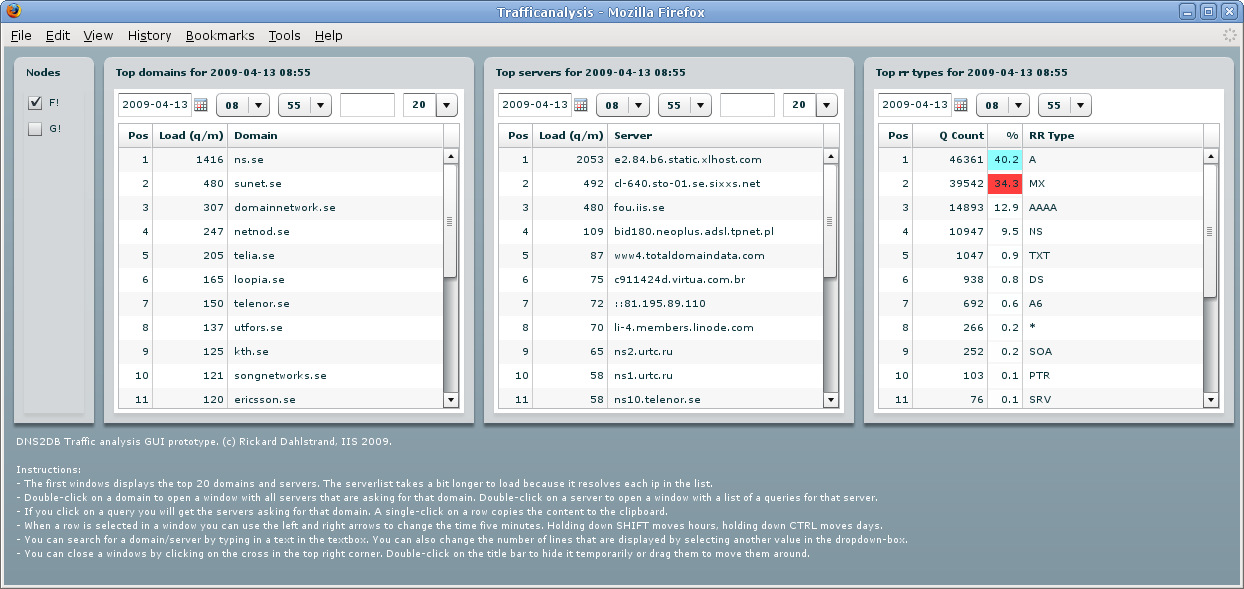
\includegraphics[width=5.0in]{../screendumps/1.png}

The flash user interface consists of a number of windows that show 
information or control which information to show about the usage of the nodes.
To use the flash user interface you need a flash enabled web browser. 

\subsection{Nodes}
The nodes window controls which nodes you currently see output 
from in the top list windows.
If a nodes name is colored green it has delivered data in response 
to the last request and if the name is colored red it has not.
Hovering the mouse over a node will pop up a small tooltip which displays status 
data about the node and the database of the selected interval such as the version 
of the dns2sqlite binary that created the database file for the interval and 
the current version of dns2db that is installed on the node.

\subsection{Filters}
Filters control what protocols and query type are currently shown. Deselecting i.e. 
udp and v4 will cause udp packets and ip v4 packets to be filtered out 
and only tcp packets over ip v6 will be shown.

\subsection{The list windows}
Common for the list windows is that they have a date, time, a filter box and a 
number of results field.
When a window is selected you can step 5 minute intervals using the left and 
right arrow keys. If SHIFT is held down the arrows key will step hours instead 
and if the CTRL key is held it will step days.
The time between the \textbf{Top domains}, \textbf{Top rr types}, 
\textbf{Top servers} and \textbf{Top repeating resolvers} windows are 
linked and always the same.

Note that loads are expressed as queries per minute and a load of 0 queries per 
minute may mean anything between 1 and 4 queries during a five minute interval.


\subsection{Top domains}
The Top domains window show the top domains ordered by queries per minute. 
Clicking on a domain in the list will open the Servers asking about [domain] 
window for that resolver.

\subsection{Top servers}
The Top servers window show the top resolvers ordered by queries per minute. 
Clicking on a resolver in the list will open the Queries from [server] window 
for that resolver.
\subsection{Top rr types}
The Top servers window show the top rr types ordered by queries per minute. 
The fields are colored according to the rrstats array in the configuration 
for the gui server. 
\subsection{Top repeating resolvers}
The Top repeating resolvers window show the top resolvers repeating the same 
query ordered by repeated queries per minute. 
\subsection{Servers asking about [domain]}
The Servers asking about [domain name] window show resolvers asking about a 
certain domain ordered by queries per minute. 
\subsection{Queries from [server]}
The Queries from [server] window show queries from a certain resolver ordered 
by queries per minute. 





\end{document}

